\documentclass[12pt,letterpaper]{exam}
\usepackage[utf8]{inputenc}
\usepackage[T1]{fontenc}
\usepackage[width=8.50in, height=11.00in, left=0.50in, right=0.50in, top=0.50in, bottom=0.50in]{geometry}

\usepackage{libertine}
\usepackage{multicol}
\usepackage[shortlabels]{enumitem}

\usepackage{booktabs}
\usepackage[table]{xcolor}

\usepackage{amssymb}
\usepackage{amsthm}
\usepackage{mathtools}
\usepackage{bbm}

\usepackage{hyperref}
\usepackage{graphicx}
%\usepackage{wrapfig}
%\usepackage{capt-of}
\usepackage{tikz}
\usepackage{subcaption}
%\usepackage{pgfplots}
%\usetikzlibrary{shapes,arrows,positioning,patterns}
%\usepackage{pythonhighlight}

%\newcommand\chapter{5}
\renewcommand{\thequestion}{\textbf{\arabic{question}}}
\renewcommand{\thepartno}{\textbf{\arabic{partno}}}
\renewcommand{\thesubpart}{\textbf{\alph{subpart}}}

\renewcommand{\questionlabel}{\thequestion.}
\renewcommand{\partlabel}{\thequestion.\thepartno)}
\renewcommand{\subpartlabel}{\thesubpart.}

%%%%%%%%%%%%%%%%%%%%%%%%%%%%%%%%%%%%%%%%%%%%%%%%%%%%%%%%%%%%%%%%%%
\newcommand{\class}{OPER 623} % This is the name of the course 
\newcommand{\assignmentname}{Exam 1} % 
\newcommand{\authorname}{Hosley, Brandon} % 
\newcommand{\workdate}{\today} % 
\printanswers % this includes the solutions sections
%%%%%%%%%%%%%%%%%%%%%%%%%%%%%%%%%%%%%%%%%%%%%%%%%%%%%%%%%%%%%%%%%%



\begin{document}
\pagestyle{plain}
\thispagestyle{empty}
\noindent
 
%%%%%%%%%%%%%%%%%%%%%%%%%%%%%%%%%%%%%%%%%%%%%%%%%%%%%%%%%%%%%%%%%%%%%%%%%%%%%%%%%%%
\noindent
\begin{tabular*}{\textwidth}{l @{\extracolsep{\fill}} r @{\extracolsep{10pt}} l}
	\textbf{\class} & \textbf{\authorname}  &\\ %Your name here instead, obviously 
	\textbf{\assignmentname } & \textbf{\workdate} & \\
\end{tabular*}\\ 
\rule{\textwidth}{2pt}
%%%%%%%%%%%%%%%%%%%%%%%%%%%%%%%% HEADER %%%%%%%%%%%%%%%%%%%%%%%%%%%%%%%%%%%%%%%%%%%

\begin{questions}
	\setcounter{question}{0}
	
	\question % 1
	\textbf{\large Computational Complexity and Transformations (30 Pts)}
	
	\begin{parts}
		% 1.1
		\part
		(5 pts) Given the following function: \(f(n) = 6n^5 + 5n^4 + 4n^3 + 3n^2 + 2n + 1\)?
		\begin{subparts}
			\subpart
			What is the Big \textbf{O} runtime for \(f(n)\)?
			\subpart
			 Prove your assertion.
		\end{subparts}
		
		\begin{solution}
			\begin{subparts}
				\subpart
				\(f(n) = \mathbf{O}(n^5)\)
				\subpart
				\begin{proof}
					This assertion is definitionally true iff there exists \(c\in\mathbb R\)
					such that \(f(n) \leq c\,n^5\).
					This \(c\) can be calculated as
					\[c \geq ( 6^5 + 5^4 + 4^3 + 3^2 + 2 + 1 )^{1/6} \approx 6.1045.\]
					Thus, \[f(n) \leq c\,n^5 \quad \forall c\geq 6.1045.\]
				\end{proof}
			\end{subparts}
		\end{solution}
		
		
		% 1.2
		\part
		(5 pts) You are given a graph \(G = (V, E)\) where \(|V| = n,\text{ and }|E| = m\). 
		You apply the following constructive heuristic to find an Independent Set: 
		Calculate the degree for all vertices \(v \in V\) and pick the \(v_i\) 
		with the lowest degree to be a member of your IS. 
		Recalculate the degree for all vertices \(v \in V\) to all vertices \(v \in V \cap v \notin\) IS
		(i.e., the degree of edges to vertices not in IS) 
		and pick the \(v_i\) with the lowest degree to be a member of your IS.
		Repeat until no new vertices can be added to your IS.
		\begin{subparts}
			\subpart
			What is the Big \textbf{O} notation run time for this Heuristic? 
			(Remember Big \textbf{O} is worst case analysis).
			\subpart
			Prove your assertion.
		\end{subparts}
		
		\begin{solution}
			\begin{subparts}
				\subpart The described heuristic would be considered \(\mathbf O(n^2)\)
				\subpart The worst case scenario occurs when the degree of every node in the graph is 0.
				In which case there will be \(n\) rounds of calculating the degree of 
				\(n-i\), \(\forall i\in n\) nodes.
				The actual number of interactions with the nodes will be
				\[\frac{n(n-1)}{2} = \frac{n^2-n}{2} = \frac{1}{2}n^2 - \frac{1}{2}n.\]
				The actual calculating of degree is linear as \(2m\) increments are counted (on the first round).
				This value is monotonically non-increasing, but the changes cannot be known a prior.
				As such
				\[f(n) \leq \mathbf{O}(n^2) \equiv c\,n^2 \quad \forall c \geq m+1.\]
				Note that this  is not the lower bound of feasible values of \(c\).
			\end{subparts}
		\end{solution}
		
		\clearpage
		% 1.3
		\part
		(10 pts) Given that Hamiltonian Cycle is in NP-Complete prove that the TSP problem is in NP-Complete. \\
		
		\textbf{Hamiltonian Cycle}: \textit{Given a, \underline{not necessarily complete}, 
			graph G = (V, E), does there exist a cycle that visits all vertices exactly once?}
		\textbf{Traveling Salesman Problem}: \textit{Given a \underline{complete} Graph G=(V,E), 
			does there exist a tour of length k or shorter?}
		\begin{subparts}
			\subpart
			Create a small but interesting instance of Hamiltonian Cycle 
			and show the transformation on that instance.
			\subpart
			Provide a general description of your valid transformation showing that TSP is in NP-Hard
			\subpart
			Show your transformation meets Tovey’s 3 criteria.
			\subpart
			Prove that TSP is in NP
		\end{subparts}
		
		\begin{solution}
			\begin{subparts}
				\subpart
				A simple example, that I find quite interesting is that all platonic solids have a solvable Hamiltonian path along their edges (red in the examples).
				
				\begin{minipage}{0.3\linewidth}				
					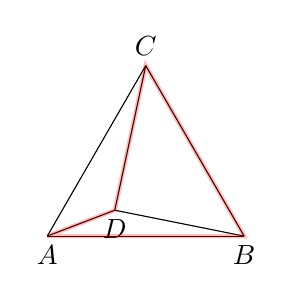
\begin{tikzpicture}[scale=1.25]
						% Define the vertices of the tetrahedron
						\coordinate[label=below:$A$] (A) at (0,0,0);
						\coordinate[label=below:$B$] (B) at (2,0,0);
						\coordinate[label=above:$C$] (C) at (1,{sqrt(3)},0);
						\coordinate[label=below:$D$] (D) at (1,{sqrt(3)/3},{sqrt(6)/3});
						
						% Draw the edges of the tetrahedron
						\draw (A) -- (B);
						\draw (A) -- (C);
						\draw (A) -- (D);
						\draw (B) -- (C);
						\draw (B) -- (D);
						\draw (C) -- (D);
						
						% Draw a Hamiltonian cycle
						\draw[ultra thick,red,opacity=0.25] (A) -- (B) -- (C) -- (D) -- (A);
					\end{tikzpicture}
				\end{minipage}
				\hfill
				\begin{minipage}{0.3\linewidth}	
					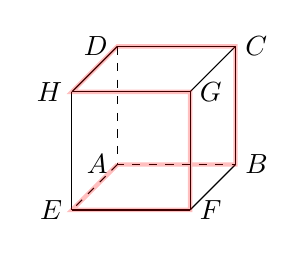
\begin{tikzpicture}[scale=1.5]
						% Define the vertices of the cube
						\coordinate[label=left:$A$] (A) at (0,0,0);
						\coordinate[label=right:$B$] (B) at (1,0,0);
						\coordinate[label=right:$C$] (C) at (1,1,0);
						\coordinate[label=left:$D$] (D) at (0,1,0);
						\coordinate[label=left:$E$] (E) at (0,0,1);
						\coordinate[label=right:$F$] (F) at (1,0,1);
						\coordinate[label=right:$G$] (G) at (1,1,1);
						\coordinate[label=left:$H$] (H) at (0,1,1);
						
						% Draw the edges of the cube
						\draw[dashed] (D) -- (A) -- (B) ;
						\draw (B) -- (C) -- (D);
						\draw (E) -- (F);
						\draw (F) -- (G) -- (H);
						\draw (H) -- (E);
						\draw[dashed] (A) -- (E);
						\draw (B) -- (F);
						\draw (C) -- (G);
						\draw (D) -- (H);
						
						% Draw a Hamiltonian cycle
						\draw[ultra thick,red,opacity=0.25] (A) -- (B) -- (C) -- (D) -- (H) -- (G) -- (F) -- (E) -- (A);
					\end{tikzpicture}
				\end{minipage}
				\hfill
				\begin{minipage}{0.3\linewidth}	
					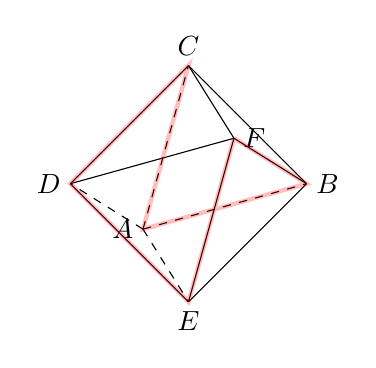
\begin{tikzpicture}[scale=1.5]
						% Define the vertices of the octahedron
						\coordinate[label=left:$A$]  (A) at (0,0,1);
						\coordinate[label=right:$B$] (B) at (1,0,0);
						\coordinate[label=above:$C$] (C) at (0,1,0);
						\coordinate[label=left:$D$]  (D) at (-1,0,0);
						\coordinate[label=below:$E$]  (E) at (0,-1,0);
						\coordinate[label=right:$F$] (F) at (0,0,-1);
						
						% Draw the edges of the octahedron
						\draw[dashed] (A) -- (B);
						\draw[dashed] (A) -- (C);
						\draw[dashed] (A) -- (D);
						\draw[dashed] (A) -- (E); 
						\draw (B) -- (C);
						\draw (C) -- (D);
						\draw (D) -- (E);
						\draw (E) -- (B);
						\draw (F) -- (B);
						\draw (F) -- (C);
						\draw (F) -- (D);
						\draw (F) -- (E);
						
						% Draw a Hamiltonian cycle
						\draw[ultra thick,red,opacity=0.25] (F) -- (B) -- (A) --  (C) -- (D) -- (E)  -- (F);
					\end{tikzpicture}
				\end{minipage} \\[1em]
				
				\begin{minipage}{0.2\linewidth}				
					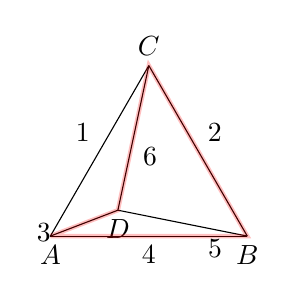
\begin{tikzpicture}[scale=1.25]
						% Define the vertices of the tetrahedron
						\coordinate[label=below:$A$] (A) at (0,0,0);
						\coordinate[label=below:$B$] (B) at (2,0,0);
						\coordinate[label=above:$C$] (C) at (1,{sqrt(3)},0);
						\coordinate[label=below:$D$] (D) at (1,{sqrt(3)/3},{sqrt(6)/3});
						
						% Draw the edges of the tetrahedron
						\draw (A) -- (B) node[pos=0.5, below] {4};
						\draw (A) -- (C) node[pos=0.5, above left] {1};
						\draw (A) -- (D) node[pos=0.15, left] {3};
						\draw (B) -- (C) node[pos=0.5, above right] {2};
						\draw (B) -- (D) node[pos=0.25, below] {5};
						\draw (C) -- (D) node[pos=0.5, below right] {6};
						
						% Draw a Hamiltonian cycle
						\draw[ultra thick,red,opacity=0.25] (A) -- (B) -- (C) -- (D) -- (A);
					\end{tikzpicture}
				\end{minipage}
				\hfill
				\begin{minipage}{0.5\linewidth}	
					The tetrahedron example can be shown as a representation of a traveling salesman problem 
					by simply assigning values to the edges. 
					However, in the case of incomplete graphs, such as our hexahedron, 
					it would otherwise be necessary to calculate the pairwise distances between unconnected nodes.
					However, even without these calculated values, the Hamiltonian cycle solution
					is a feasible solution to the TSP.
					
				\end{minipage}
				\hfill
				\begin{minipage}{0.225\linewidth}	
					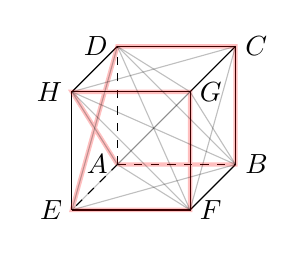
\begin{tikzpicture}[scale=1.5]
						% Define the vertices of the cube
						\coordinate[label=left:$A$] (A) at (0,0,0);
						\coordinate[label=right:$B$] (B) at (1,0,0);
						\coordinate[label=right:$C$] (C) at (1,1,0);
						\coordinate[label=left:$D$] (D) at (0,1,0);
						\coordinate[label=left:$E$] (E) at (0,0,1);
						\coordinate[label=right:$F$] (F) at (1,0,1);
						\coordinate[label=right:$G$] (G) at (1,1,1);
						\coordinate[label=left:$H$] (H) at (0,1,1);
						
						% Draw the edges of the cube
						\draw[dashed] (A) -- (B);
						\draw[dashed] (A) -- (D);
						\draw (B) -- (C) -- (D);
						\draw (E) -- (F) -- (G) -- (H) -- (E);
						\draw[dashed] (A) -- (E);
						\draw (B) -- (F);
						\draw (C) -- (G);
						\draw (D) -- (H);
						
						% Draw a Hamiltonian cycle
						\draw[ultra thick,red,opacity=0.25] (A) -- (B) -- (C) -- (D) -- (E) -- (F) -- (G)  -- (H) -- (A);
						
						% Draw additional routes
						\draw[opacity=0.25] (A) -- (C);
						\draw[opacity=0.25] (A) -- (F);
						\draw[opacity=0.25] (A) -- (H);
						\draw[opacity=0.25] (B) -- (D);
						\draw[opacity=0.25] (B) -- (E);
						\draw[opacity=0.25] (B) -- (G);
						\draw[opacity=0.25] (B) -- (H);
						\draw[opacity=0.25] (C) -- (F);
						\draw[opacity=0.25] (C) -- (H);
						\draw[opacity=0.25] (D) -- (E);
						\draw[opacity=0.25] (D) -- (F);
						\draw[opacity=0.25] (D) -- (G);
						\draw[opacity=0.25] (E) -- (G);
						\draw[opacity=0.25] (F) -- (H);
					\end{tikzpicture}
				\end{minipage} \\[1em]
				
				
				\subpart
				
				Given any instance of a Hamiltonian cycle problem,
				\begin{enumerate}
					\item First, complete the graph (as illustrated in the hexahedron example)
					\item Calculate a value for each edge (as illustrated in the tetrahedron example)
				\end{enumerate}
				
				Then, because the TSP has \textbf{at least} as many edges as a HCP, it will always be 
				at least as difficult as the corresponding HCP.
								
				
				\subpart
				For any solution \(S\);
				
				\begin{enumerate}
					\item
					Every Hamiltonian Circuit solution is such that
					
					\(G(V) \notin S(V) = \{\emptyset\} \), and
	
					\(S(E_i) \neq S(E_j) \quad \forall\ i\neq j\).
				
					As such, any circuit solution is a feasible solution to the TSP	
					
					\item
					The constraints listed above, being necessary for a feasible TSP solution,
					it can be converted into an HCP solution. 
					
					The values assigned to the edges may be dropped and any
					\(G(E) \notin S(E)\)
					may optionally be removed as well.
					
					\item
					Conversion from an HCP to a TSP requires completing the graph, 
					which takes \(leq V^2\) operations;
					And assigning values to each edge, which takes \(E^*\) operations
					where \(E^*\) represents the edges of the newly completed graph.
					
					Thus, the conversion takes at most \(V^2 + E^*\) or \(2V^2\) operations.
					This puts the function into the \(\mathbf{O}(n^2)\) range.
					
				\end{enumerate}
				
				
				\subpart
				
				\begin{proof}
				Verifying the feasibility of a solution \(S\) means verifying
				\(G(V) \notin S(V) = \{\emptyset\} \) and 			
				\(S(E_i) \neq S(E_j) \quad \forall\ i\neq j\),
				which would require \(S(V) + S(E) = 2V\) operations.
				To verify the decision portion of the TSP is
				\(\sum_{e_i\in S(E)}e_i \leq k\) 
				where \(e_i\) represents the value of the edge.
				Thus solution verification can be done in linear time.
				
				Part \textbf{c.} demonstrated the relationship between feasible answers
				of TSP and a known NP-complete problem, and that the transition between
				the two can be completed in polynomial time. 
				The validity of this transformation was also shown to meet Tovey's 3 criteria in part \textbf{c}.
				
				The increased difficulty for TSP can be demonstrated by accounting for the fact that
				every feasible TSP solution is in HCP, but not every feasible solution
				will have a total value of less than \(k\).
				\end{proof}				
				
				
			\end{subparts}
			
			
		\end{solution}
		
		
		% 1.4
		\part
		(10 pts) Prove that the problem of determining if a, not necessarily complete, 
		graph \textbf{G =(V,E)} yields a Spanning Tree where all vertices in the 
		spanning tree have degree 2 or less, is in NP-Complete.
		\begin{solution}
		
		\end{solution}
	\end{parts}		
%%%%%%%%%%%%%%%%%%%%%%%%%%%%%%%%%%%%%%%%%%%%%%%%%%%%%%%%%%%%%
	
	
	\question % 2
	\textbf{\large Constructive Heuristics (30 Pts)}
	Consider the 8 queens problem:
	\begin{parts}
		\part 
		(15 Pts) Propose a constructive heuristic to place all 8 queens 
		which aims to minimize infeasibility of placement.
		\part 
		(5 Pts) Provide a step by step example to illustrate your heuristic.
		\part 
		(5 pts) Critique your heuristic based on the criteria presented in Lesson 4 
		(Features of a Good Heuristic). Provide pros and cons.
		\part 
		(5 Pts) What are the initial steps to code your heuristic, specifically: 
		In a computer code how would you encode the queen locations and track growth in different queens attack paths?
	\end{parts}
	
	\begin{solution}
		
	\end{solution}
%%%%%%%%%%%%%%%%%%%%%%%%%%%%%%%%%%%%%%%%%%%%%%%%%%%%%%%%%%%%%
	
	
	\question % 3
	\textbf{\large Local Search Heuristics (30 Pts)}
	Consider the classic children’s shuffle puzzle, where you are given a picture and 
	need to shuffle tiles to make the picture look correct. An example is shown below. 
	(Note that by physical construction the only pieces that can move are those adjacent to the “missing” tile.)
	\includegraphics[width=0.27\linewidth]{"Screenshot 2023-11-09 at 7.55.50 PM"}
	\begin{parts}
		\part
		(20 Pts) Propose a local search heuristic to solve the puzzle. 
		(Recall local search heuristics do not have memory, and cannot use global information). 
		Ensure you address the following in your description.
		\begin{subparts}
			\subpart What is your “objective function”?
			\subpart What is your definition of a move?
			\subpart How do you select a neighbor?
		\end{subparts}
		\begin{solution}
			\begin{subparts}
				\subpart
				
				Instead of using the labeling system presented in part \textbf{3.2}, 
				I have elected to use coordinates to identify cells \(C\) and tiles \(T\).
				For an \(m\) by \(n\) board our objective function is				
				
				\[\min \sum_{i=0}^{mn} 2^{|T_{i,x} - C_{i,x}|} + 2^{|T_{i,y} - C_{i,y}|} .\]
				
				The reason for the exponent will be explained further in section \textbf{c}.
				It is not necessary for evaluating the overall state of the board,
				but it is presented this way to be consistent with local evaluation.
				
				\subpart
				A move consists of taking any neighboring tile, moving it into the currently empty space,
				and thus the tile's previously occupied space becomes the new empty space.
				
				\subpart
				From among the neighbors of the empty cell, the value of each 
				candidate tile is evaluated using both its current cell and the empty cell. 
				The neighbor with the biggest decrease in value is selected to move to the empty cell.

				A termination state is necessary. 
				For this we assume that the final coordinates of the empty cell are known.
				Once the empty cell is in the appropriate place \textit{and} all potential moves
				represent a decrease in the objective function value the heuristic terminates.
				
				If the empty cell is not in the appropriate place and none of the candidate neighbors
				provide an improvement from moving,	then the heuristic continues by selecting
				the move that represents the lowest increase in the objective function.
				
				Example provided in problem \textbf{3.2}.
			\end{subparts}			
		\end{solution}
		
		
		\part
		(10 Pts) Provide a concrete 3 x 3 example to illustrate your heuristic. 
		Show all necessary iterations to achieve local optima. 
		Note: Your 3 x 3 example can just use the numbers 1-8 for ease of reference.
		\begin{solution}
			
			
			\begin{minipage}{0.2\linewidth}	
				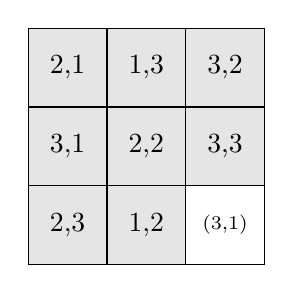
\begin{tikzpicture}
					% Define the grid
					\foreach \x in {0,1,2} \foreach \y in {0,1,2} \draw (\x,\y) rectangle ++(1,1);
					% Add labels to the cells
					\foreach \x in {1,2,3} \foreach \y in {1,2,3}{
						\node at (\x-0.5,\y-0.5) {\scriptsize (\x,\y)};} 				
					% Create Tiles
					\draw[fill=gray!20] (0,0) rectangle ++(1,1) node[midway] {2,3};
					\draw[fill=gray!20] (1,0) rectangle ++(1,1) node[midway] {1,2};
					%\draw[fill=gray!20] (2,0) rectangle ++(1,1) node[midway] {2};
					\draw[fill=gray!20] (0,1) rectangle ++(1,1) node[midway] {3,1};
					\draw[fill=gray!20] (1,1) rectangle ++(1,1) node[midway] {2,2};
					\draw[fill=gray!20] (2,1) rectangle ++(1,1) node[midway] {3,3};
					\draw[fill=gray!20] (0,2) rectangle ++(1,1) node[midway] {2,1};
					\draw[fill=gray!20] (1,2) rectangle ++(1,1) node[midway] {1,3};
					\draw[fill=gray!20] (2,2) rectangle ++(1,1) node[midway] {3,2};
				\end{tikzpicture}
			\end{minipage}
			%
			\begin{minipage}{0.2\linewidth}	
				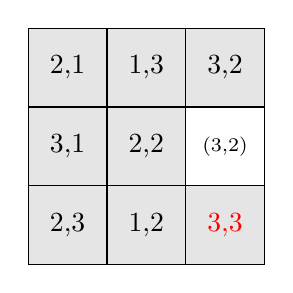
\begin{tikzpicture}
					% Define the grid
					\foreach \x in {0,1,2} \foreach \y in {0,1,2} \draw (\x,\y) rectangle ++(1,1);
					% Add labels to the cells
					\foreach \x in {1,2,3} \foreach \y in {1,2,3}{
						\node at (\x-0.5,\y-0.5) {\scriptsize (\x,\y)};} 				
					% Create Tiles
					\draw[fill=gray!20] (0,0) rectangle ++(1,1) node[midway] {2,3};
					\draw[fill=gray!20] (1,0) rectangle ++(1,1) node[midway] {1,2};
					\draw[fill=gray!20] (2,0) rectangle ++(1,1) node[midway] {\textcolor{red}{3,3}};
					\draw[fill=gray!20] (0,1) rectangle ++(1,1) node[midway] {3,1};
					\draw[fill=gray!20] (1,1) rectangle ++(1,1) node[midway] {2,2};
					%\draw[fill=gray!20] (2,1) rectangle ++(1,1) node[midway] {3,3};
					\draw[fill=gray!20] (0,2) rectangle ++(1,1) node[midway] {2,1};
					\draw[fill=gray!20] (1,2) rectangle ++(1,1) node[midway] {1,3};
					\draw[fill=gray!20] (2,2) rectangle ++(1,1) node[midway] {3,2};
				\end{tikzpicture}
			\end{minipage}
			%
			\begin{minipage}{0.2\linewidth}	
				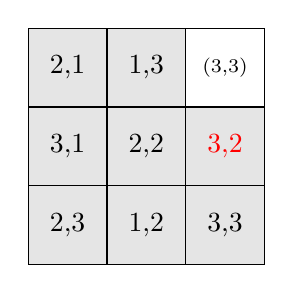
\begin{tikzpicture}
					% Define the grid
					\foreach \x in {0,1,2} \foreach \y in {0,1,2} \draw (\x,\y) rectangle ++(1,1);
					% Add labels to the cells
					\foreach \x in {1,2,3} \foreach \y in {1,2,3}{
						\node at (\x-0.5,\y-0.5) {\scriptsize (\x,\y)};} 				
					% Create Tiles
					\draw[fill=gray!20] (0,0) rectangle ++(1,1) node[midway] {2,3};
					\draw[fill=gray!20] (1,0) rectangle ++(1,1) node[midway] {1,2};
					\draw[fill=gray!20] (2,0) rectangle ++(1,1) node[midway] {3,3};
					\draw[fill=gray!20] (0,1) rectangle ++(1,1) node[midway] {3,1};
					\draw[fill=gray!20] (1,1) rectangle ++(1,1) node[midway] {2,2};
					\draw[fill=gray!20] (2,1) rectangle ++(1,1) node[midway] {\textcolor{red}{3,2}};
					\draw[fill=gray!20] (0,2) rectangle ++(1,1) node[midway] {2,1};
					\draw[fill=gray!20] (1,2) rectangle ++(1,1) node[midway] {1,3};
					%\draw[fill=gray!20] (2,2) rectangle ++(1,1) node[midway] {3,2};
				\end{tikzpicture}
			\end{minipage}
			%
			\begin{minipage}{0.2\linewidth}	
				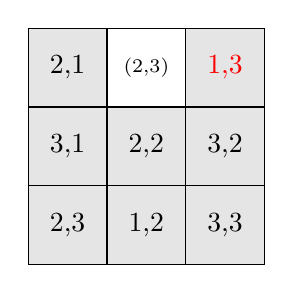
\begin{tikzpicture}
					% Define the grid
					\foreach \x in {0,1,2} \foreach \y in {0,1,2} \draw (\x,\y) rectangle ++(1,1);
					% Add labels to the cells
					\foreach \x in {1,2,3} \foreach \y in {1,2,3}{
						\node at (\x-0.5,\y-0.5) {\scriptsize (\x,\y)};} 				
					% Create Tiles
					\draw[fill=gray!20] (0,0) rectangle ++(1,1) node[midway] {2,3};
					\draw[fill=gray!20] (1,0) rectangle ++(1,1) node[midway] {1,2};
					\draw[fill=gray!20] (2,0) rectangle ++(1,1) node[midway] {3,3};
					\draw[fill=gray!20] (0,1) rectangle ++(1,1) node[midway] {3,1};
					\draw[fill=gray!20] (1,1) rectangle ++(1,1) node[midway] {2,2};
					\draw[fill=gray!20] (2,1) rectangle ++(1,1) node[midway] {3,2};
					\draw[fill=gray!20] (0,2) rectangle ++(1,1) node[midway] {2,1};
					%\draw[fill=gray!20] (1,2) rectangle ++(1,1) node[midway] {1,3};
					\draw[fill=gray!20] (2,2) rectangle ++(1,1) node[midway] {\textcolor{red}{1,3}};
				\end{tikzpicture}
			\end{minipage}
			%
			\begin{minipage}{0.2\linewidth}	
				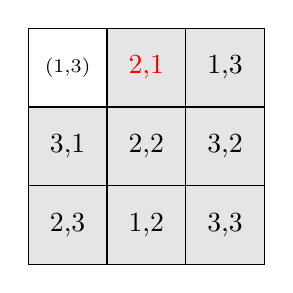
\begin{tikzpicture}
					% Define the grid
					\foreach \x in {0,1,2} \foreach \y in {0,1,2} \draw (\x,\y) rectangle ++(1,1);
					% Add labels to the cells
					\foreach \x in {1,2,3} \foreach \y in {1,2,3}{
						\node at (\x-0.5,\y-0.5) {\scriptsize (\x,\y)};} 				
					% Create Tiles
					\draw[fill=gray!20] (0,0) rectangle ++(1,1) node[midway] {2,3};
					\draw[fill=gray!20] (1,0) rectangle ++(1,1) node[midway] {1,2};
					\draw[fill=gray!20] (2,0) rectangle ++(1,1) node[midway] {3,3};
					\draw[fill=gray!20] (0,1) rectangle ++(1,1) node[midway] {3,1};
					\draw[fill=gray!20] (1,1) rectangle ++(1,1) node[midway] {2,2};
					\draw[fill=gray!20] (2,1) rectangle ++(1,1) node[midway] {3,2};
					%\draw[fill=gray!20] (0,2) rectangle ++(1,1) node[midway] {2,1};
					\draw[fill=gray!20] (1,2) rectangle ++(1,1) node[midway] {\textcolor{red}{2,1}};
					\draw[fill=gray!20] (2,2) rectangle ++(1,1) node[midway] {1,3};
				\end{tikzpicture}
			\end{minipage}
			\\[1em]
			\begin{minipage}{0.2\linewidth}	
				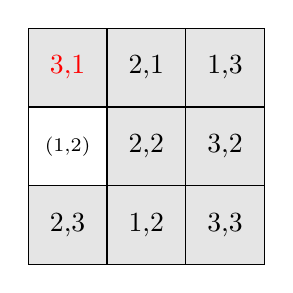
\begin{tikzpicture}
					% Define the grid
					\foreach \x in {0,1,2} \foreach \y in {0,1,2} \draw (\x,\y) rectangle ++(1,1);
					% Add labels to the cells
					\foreach \x in {1,2,3} \foreach \y in {1,2,3}{
						\node at (\x-0.5,\y-0.5) {\scriptsize (\x,\y)};} 				
					% Create Tiles
					\draw[fill=gray!20] (0,0) rectangle ++(1,1) node[midway] {2,3};
					\draw[fill=gray!20] (1,0) rectangle ++(1,1) node[midway] {1,2};
					\draw[fill=gray!20] (2,0) rectangle ++(1,1) node[midway] {3,3};
					%\draw[fill=gray!20] (0,1) rectangle ++(1,1) node[midway] {3,1};
					\draw[fill=gray!20] (1,1) rectangle ++(1,1) node[midway] {2,2};
					\draw[fill=gray!20] (2,1) rectangle ++(1,1) node[midway] {3,2};
					\draw[fill=gray!20] (0,2) rectangle ++(1,1) node[midway] {\textcolor{red}{3,1}};
					\draw[fill=gray!20] (1,2) rectangle ++(1,1) node[midway] {2,1};
					\draw[fill=gray!20] (2,2) rectangle ++(1,1) node[midway] {1,3};
				\end{tikzpicture}
			\end{minipage}
			%
			\begin{minipage}{0.2\linewidth}	
				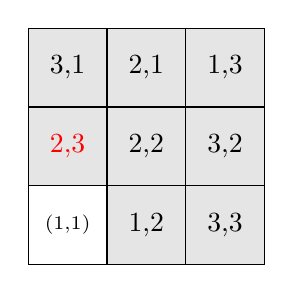
\begin{tikzpicture}
					% Define the grid
					\foreach \x in {0,1,2} \foreach \y in {0,1,2} \draw (\x,\y) rectangle ++(1,1);
					% Add labels to the cells
					\foreach \x in {1,2,3} \foreach \y in {1,2,3}{
						\node at (\x-0.5,\y-0.5) {\scriptsize (\x,\y)};} 				
					% Create Tiles
					%\draw[fill=gray!20] (0,0) rectangle ++(1,1) node[midway] {2,3};
					\draw[fill=gray!20] (1,0) rectangle ++(1,1) node[midway] {1,2};
					\draw[fill=gray!20] (2,0) rectangle ++(1,1) node[midway] {3,3};
					\draw[fill=gray!20] (0,1) rectangle ++(1,1) node[midway] {\textcolor{red}{2,3}};
					\draw[fill=gray!20] (1,1) rectangle ++(1,1) node[midway] {2,2};
					\draw[fill=gray!20] (2,1) rectangle ++(1,1) node[midway] {3,2};
					\draw[fill=gray!20] (0,2) rectangle ++(1,1) node[midway] {3,1};
					\draw[fill=gray!20] (1,2) rectangle ++(1,1) node[midway] {2,1};
					\draw[fill=gray!20] (2,2) rectangle ++(1,1) node[midway] {1,3};
				\end{tikzpicture}
			\end{minipage}
			%
			\begin{minipage}{0.2\linewidth}	
				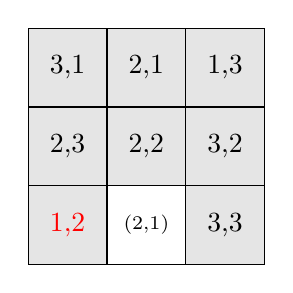
\begin{tikzpicture}
					% Define the grid
					\foreach \x in {0,1,2} \foreach \y in {0,1,2} \draw (\x,\y) rectangle ++(1,1);
					% Add labels to the cells
					\foreach \x in {1,2,3} \foreach \y in {1,2,3}{
						\node at (\x-0.5,\y-0.5) {\scriptsize (\x,\y)};} 				
					% Create Tiles
					\draw[fill=gray!20] (0,0) rectangle ++(1,1) node[midway] {\textcolor{red}{1,2}};
					%\draw[fill=gray!20] (1,0) rectangle ++(1,1) node[midway] {1,2};
					\draw[fill=gray!20] (2,0) rectangle ++(1,1) node[midway] {3,3};
					\draw[fill=gray!20] (0,1) rectangle ++(1,1) node[midway] {2,3};
					\draw[fill=gray!20] (1,1) rectangle ++(1,1) node[midway] {2,2};
					\draw[fill=gray!20] (2,1) rectangle ++(1,1) node[midway] {3,2};
					\draw[fill=gray!20] (0,2) rectangle ++(1,1) node[midway] {3,1};
					\draw[fill=gray!20] (1,2) rectangle ++(1,1) node[midway] {2,1};
					\draw[fill=gray!20] (2,2) rectangle ++(1,1) node[midway] {1,3};
				\end{tikzpicture}
			\end{minipage}
			%
			\begin{minipage}{0.2\linewidth}	
				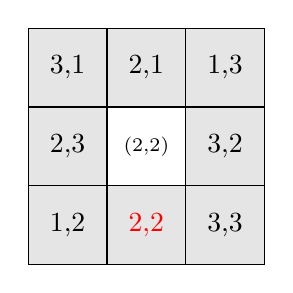
\begin{tikzpicture}
					% Define the grid
					\foreach \x in {0,1,2} \foreach \y in {0,1,2} \draw (\x,\y) rectangle ++(1,1);
					% Add labels to the cells
					\foreach \x in {1,2,3} \foreach \y in {1,2,3}{
						\node at (\x-0.5,\y-0.5) {\scriptsize (\x,\y)};} 				
					% Create Tiles
					\draw[fill=gray!20] (0,0) rectangle ++(1,1) node[midway] {1,2};
					\draw[fill=gray!20] (1,0) rectangle ++(1,1) node[midway] {\textcolor{red}{2,2}};
					\draw[fill=gray!20] (2,0) rectangle ++(1,1) node[midway] {3,3};
					\draw[fill=gray!20] (0,1) rectangle ++(1,1) node[midway] {2,3};
					%\draw[fill=gray!20] (1,1) rectangle ++(1,1) node[midway] {2,2};
					\draw[fill=gray!20] (2,1) rectangle ++(1,1) node[midway] {3,2};
					\draw[fill=gray!20] (0,2) rectangle ++(1,1) node[midway] {3,1};
					\draw[fill=gray!20] (1,2) rectangle ++(1,1) node[midway] {2,1};
					\draw[fill=gray!20] (2,2) rectangle ++(1,1) node[midway] {1,3};
				\end{tikzpicture}
			\end{minipage}
			%
			\begin{minipage}{0.2\linewidth}	
				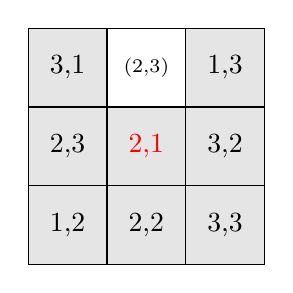
\begin{tikzpicture}
					% Define the grid
					\foreach \x in {0,1,2} \foreach \y in {0,1,2} \draw (\x,\y) rectangle ++(1,1);
					% Add labels to the cells
					\foreach \x in {1,2,3} \foreach \y in {1,2,3}{
						\node at (\x-0.5,\y-0.5) {\scriptsize (\x,\y)};} 				
					% Create Tiles
					\draw[fill=gray!20] (0,0) rectangle ++(1,1) node[midway] {1,2};
					\draw[fill=gray!20] (1,0) rectangle ++(1,1) node[midway] {2,2};
					\draw[fill=gray!20] (2,0) rectangle ++(1,1) node[midway] {3,3};
					\draw[fill=gray!20] (0,1) rectangle ++(1,1) node[midway] {2,3};
					\draw[fill=gray!20] (1,1) rectangle ++(1,1) node[midway] {\textcolor{red}{2,1}};
					\draw[fill=gray!20] (2,1) rectangle ++(1,1) node[midway] {3,2};
					\draw[fill=gray!20] (0,2) rectangle ++(1,1) node[midway] {3,1};
					%\draw[fill=gray!20] (1,2) rectangle ++(1,1) node[midway] {2,1};
					\draw[fill=gray!20] (2,2) rectangle ++(1,1) node[midway] {1,3};
				\end{tikzpicture}
			\end{minipage}
			\\[1em]
			\begin{minipage}{0.2\linewidth}	
				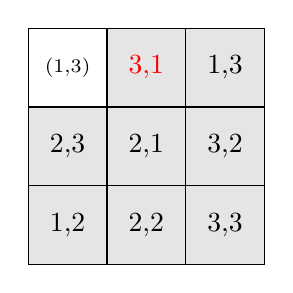
\begin{tikzpicture}
					% Define the grid
					\foreach \x in {0,1,2} \foreach \y in {0,1,2} \draw (\x,\y) rectangle ++(1,1);
					% Add labels to the cells
					\foreach \x in {1,2,3} \foreach \y in {1,2,3}{
						\node at (\x-0.5,\y-0.5) {\scriptsize (\x,\y)};} 				
					% Create Tiles
					\draw[fill=gray!20] (0,0) rectangle ++(1,1) node[midway] {1,2};
					\draw[fill=gray!20] (1,0) rectangle ++(1,1) node[midway] {2,2};
					\draw[fill=gray!20] (2,0) rectangle ++(1,1) node[midway] {3,3};
					\draw[fill=gray!20] (0,1) rectangle ++(1,1) node[midway] {2,3};
					\draw[fill=gray!20] (1,1) rectangle ++(1,1) node[midway] {2,1};
					\draw[fill=gray!20] (2,1) rectangle ++(1,1) node[midway] {3,2};
					%\draw[fill=gray!20] (0,2) rectangle ++(1,1) node[midway] {3,1};
					\draw[fill=gray!20] (1,2) rectangle ++(1,1) node[midway] {\textcolor{red}{3,1}};
					\draw[fill=gray!20] (2,2) rectangle ++(1,1) node[midway] {1,3};
				\end{tikzpicture}
			\end{minipage}
			%
			\begin{minipage}{0.2\linewidth}	
				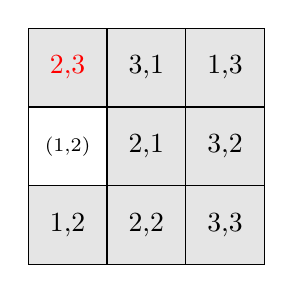
\begin{tikzpicture}
					% Define the grid
					\foreach \x in {0,1,2} \foreach \y in {0,1,2} \draw (\x,\y) rectangle ++(1,1);
					% Add labels to the cells
					\foreach \x in {1,2,3} \foreach \y in {1,2,3}{
						\node at (\x-0.5,\y-0.5) {\scriptsize (\x,\y)};} 				
					% Create Tiles
					\draw[fill=gray!20] (0,0) rectangle ++(1,1) node[midway] {1,2};
					\draw[fill=gray!20] (1,0) rectangle ++(1,1) node[midway] {2,2};
					\draw[fill=gray!20] (2,0) rectangle ++(1,1) node[midway] {3,3};
					%\draw[fill=gray!20] (0,1) rectangle ++(1,1) node[midway] {2,3};
					\draw[fill=gray!20] (1,1) rectangle ++(1,1) node[midway] {2,1};
					\draw[fill=gray!20] (2,1) rectangle ++(1,1) node[midway] {3,2};
					\draw[fill=gray!20] (0,2) rectangle ++(1,1) node[midway] {\textcolor{red}{2,3}};
					\draw[fill=gray!20] (1,2) rectangle ++(1,1) node[midway] {3,1};
					\draw[fill=gray!20] (2,2) rectangle ++(1,1) node[midway] {1,3};
				\end{tikzpicture}
			\end{minipage}
			%
			\begin{minipage}{0.2\linewidth}	
				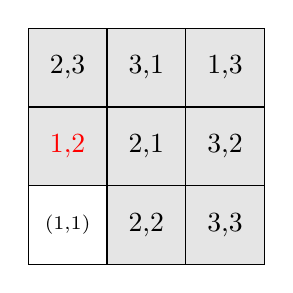
\begin{tikzpicture}
					% Define the grid
					\foreach \x in {0,1,2} \foreach \y in {0,1,2} \draw (\x,\y) rectangle ++(1,1);
					% Add labels to the cells
					\foreach \x in {1,2,3} \foreach \y in {1,2,3}{
						\node at (\x-0.5,\y-0.5) {\scriptsize (\x,\y)};} 				
					% Create Tiles
					%\draw[fill=gray!20] (0,0) rectangle ++(1,1) node[midway] {1,2};
					\draw[fill=gray!20] (1,0) rectangle ++(1,1) node[midway] {2,2};
					\draw[fill=gray!20] (2,0) rectangle ++(1,1) node[midway] {3,3};
					\draw[fill=gray!20] (0,1) rectangle ++(1,1) node[midway] {\textcolor{red}{1,2}};
					\draw[fill=gray!20] (1,1) rectangle ++(1,1) node[midway] {2,1};
					\draw[fill=gray!20] (2,1) rectangle ++(1,1) node[midway] {3,2};
					\draw[fill=gray!20] (0,2) rectangle ++(1,1) node[midway] {2,3};
					\draw[fill=gray!20] (1,2) rectangle ++(1,1) node[midway] {3,1};
					\draw[fill=gray!20] (2,2) rectangle ++(1,1) node[midway] {1,3};
				\end{tikzpicture}
			\end{minipage}
			%
			\begin{minipage}{0.2\linewidth}	
				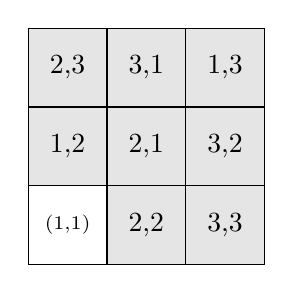
\begin{tikzpicture}
					% Define the grid
					\foreach \x in {0,1,2} \foreach \y in {0,1,2} \draw (\x,\y) rectangle ++(1,1);
					% Add labels to the cells
					\foreach \x in {1,2,3} \foreach \y in {1,2,3}{
						\node at (\x-0.5,\y-0.5) {\scriptsize (\x,\y)};} 				
					% Create Tiles
					%\draw[fill=gray!20] (0,0) rectangle ++(1,1) node[midway] {1,2};
					\draw[fill=gray!20] (1,0) rectangle ++(1,1) node[midway] {2,2};
					\draw[fill=gray!20] (2,0) rectangle ++(1,1) node[midway] {3,3};
					\draw[fill=gray!20] (0,1) rectangle ++(1,1) node[midway] {1,2};
					\draw[fill=gray!20] (1,1) rectangle ++(1,1) node[midway] {2,1};
					\draw[fill=gray!20] (2,1) rectangle ++(1,1) node[midway] {3,2};
					\draw[fill=gray!20] (0,2) rectangle ++(1,1) node[midway] {2,3};
					\draw[fill=gray!20] (1,2) rectangle ++(1,1) node[midway] {3,1};
					\draw[fill=gray!20] (2,2) rectangle ++(1,1) node[midway] {1,3};
				\end{tikzpicture}
			\end{minipage}
			%
			\begin{minipage}{0.2\linewidth}	
				\begin{tikzpicture}
					% Define the grid
				%	\foreach \x in {0,1,2} \foreach \y in {0,1,2} \draw (\x,\y) rectangle ++(1,1);
				%	% Add labels to the cells
				%	\foreach \x in {1,2,3} \foreach \y in {1,2,3}{
				%		\node at (\x-0.5,\y-0.5) {\scriptsize (\x,\y)};} 				
					% Create Tiles
					%\draw[fill=gray!20] (0,0) rectangle ++(1,1) node[midway] {1,2};
				%	\draw[fill=gray!20] (1,0) rectangle ++(1,1) node[midway] {2,2};
				%	\draw[fill=gray!20] (2,0) rectangle ++(1,1) node[midway] {3,3};
				%	\draw[fill=gray!20] (0,1) rectangle ++(1,1) node[midway] {1,2};
				%	\draw[fill=gray!20] (1,1) rectangle ++(1,1) node[midway] {2,1};
				%	\draw[fill=gray!20] (2,1) rectangle ++(1,1) node[midway] {3,2};
				%	\draw[fill=gray!20] (0,2) rectangle ++(1,1) node[midway] {2,3};
				%	\draw[fill=gray!20] (1,2) rectangle ++(1,1) node[midway] {3,1};
				%	\draw[fill=gray!20] (2,2) rectangle ++(1,1) node[midway] {1,3};
				\end{tikzpicture}
			\end{minipage}
			\\
			
			In the last, the empty space is in the position that it would be for the properly solved puzzle.
			The two adjacent tiles both represent an increase in their contribution to the objective function.
			While it is possible that continuing the heuristic would improve the result,
			there had to be some terminating criteria that did not have memory.
			
			In this particular local minima we have a state in which 7/9 of the tiles are in 
			either the correct row or correct column. 
			
		\end{solution}
		
	\end{parts}
%%%%%%%%%%%%%%%%%%%%%%%%%%%%%%%%%%%%%%%%%%%%%%%%%%%%%%%%%%%%%
	
	
	\question % 4
	\textbf{\large Coding (10 Pts)}
	\begin{parts}
		\part
		Using the software of your choice write an implementation of the GRASP 
		Heuristic for the Traveling Salesman Problem (TSP).
		\begin{subparts}
			\subpart
			Ensure that your code runs the lab data example, and is robust enough that if the TSP instance within
			that file were replaced by a larger/different TSP instance your code still runs correctly.
			\subpart
			Ensure you comment your code \underline{thoroughly}.
			\subpart
			You are free to recycle sections of the Nearest Neighbor and/or 2OPT code provided in labs as desired.
		\end{subparts}
		\begin{solution}
			
		\end{solution}
	\end{parts}
%%%%%%%%%%%%%%%%%%%%%%%%%%%%%%%%%%%%%%%%%%%%%%%%%%%%%%%%%%%%%
	
	
	\question % 5
	\textbf{\large Extra Credit (5 Pts)}
	\begin{subparts}
		\subpart
		Create a transformation, associated explanation, and proof of validity, 
		that enables the transformation of any instance of Sudoku to an 
		instance of Graph Coloring (Aka Chromatic Number).
	\end{subparts}
	\begin{solution}
		
	\end{solution}
	%%%%%%%%%%%%%%%%%%%%%%%%%%%%%%%%%%%%%%%%%%%%%%%%%%%%%%%%%%%%%
	
\end{questions}
\end{document}